\documentclass{article}
\usepackage{tikz}
\usetikzlibrary{decorations.markings}

\begin{document}

\begin{figure}
\centering
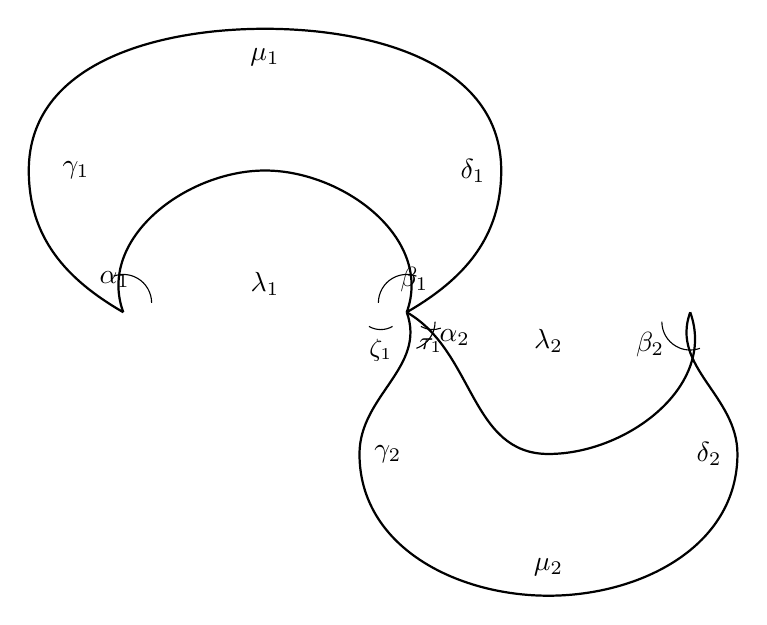
\begin{tikzpicture}[scale=1.2]
    % First spherical linkage (upper)
    \draw[thick] (0,0) to[out=110, in=180] (1.5,1.5) to[out=0, in=70] (3,0);
    \draw[thick] (0,0) to[out=150, in=270] (-1,1.5) to[out=90, in=180] (1.5,3) to[out=0, in=90] (4,1.5) to[out=270, in=30] (3,0);
    
    % Second spherical linkage (lower)
    \draw[thick] (3,0) to[out=330, in=180] (4.5,-1.5) to[out=0, in=290] (6,0);
    \draw[thick] (3,0) to[out=290, in=90] (2.5,-1.5) to[out=270, in=180] (4.5,-3) to[out=0, in=270] (6.5,-1.5) to[out=90, in=250] (6,0);
    
    % Angle markers for first linkage
    \draw (0.3,0.1) arc (0:110:0.3) node[left, pos=0.5] {$\alpha_1$};
    \draw (2.7,0.1) arc (180:70:0.3) node[right, pos=0.5] {$\beta_1$};
    
    % Angle markers for second linkage
    \draw (3.3,-0.1) arc (0:-70:0.3) node[right, pos=0.5] {$\alpha_2$};
    \draw (5.7,-0.1) arc (180:290:0.3) node[left, pos=0.5] {$\beta_2$};
    
    % Angle markers for gap
    \draw (3.15,-0.15) arc (240:290:0.25) node[below, pos=0.5, font=\small] {$\tau_1$};
    \draw (2.85,-0.15) arc (300:240:0.25) node[below, pos=0.5, font=\small] {$\zeta_1$};
    
    % Labels for first linkage sides
    \node at (-0.5,1.5) {$\gamma_1$};
    \node at (1.5,2.7) {$\mu_1$};
    \node at (3.7,1.5) {$\delta_1$};
    \node at (1.5,0.3) {$\lambda_1$};
    
    % Labels for second linkage sides
    \node at (2.8,-1.5) {$\gamma_2$};
    \node at (4.5,-2.7) {$\mu_2$};
    \node at (6.2,-1.5) {$\delta_2$};
    \node at (4.5,-0.3) {$\lambda_2$};
    
\end{tikzpicture}
\caption{Left: Partial and whole spherical linkage of a mesh in Fig.~\ref{sqmesh}, $(\lambda_i, \gamma_i, \mu_i, \delta_i,\alpha_i,\beta_i)$ and $(\lambda_i', \gamma_i', \mu_i', \delta_i',\alpha_i',\beta_i')$ are complementary to $\pi$ respectively, the gap between $\beta_1$ and $\alpha_2$ is caused by $\tau_1$ and $\zeta_1$.}
\label{fig:spherical_linkage}
\end{figure}

\end{document}